\let\negmedspace\undefined
\let\negthickspace\undefined
\documentclass[journal]{IEEEtran}
\usepackage[a5paper, margin=10mm, onecolumn]{geometry}
%\usepackage{lmodern} % Ensure lmodern is loaded for pdflatex
\usepackage{tfrupee} % Include tfrupee package

\setlength{\headheight}{1cm} % Set the height of the header box
\setlength{\headsep}{0mm}     % Set the distance between the header box and the top of the text

\usepackage{gvv-book}
\usepackage{gvv}
\usepackage{cite}
\usepackage{amsmath,amssymb,amsfonts,amsthm,mathtools}
\usepackage{algorithmic}
\usepackage{graphicx}
\usepackage{textcomp}
\usepackage{xcolor}
\usepackage{txfonts}
\usepackage{listings}
\usepackage{enumitem}
\usepackage{mathtools}
\usepackage{gensymb}
\usepackage{comment}
\usepackage[breaklinks=true]{hyperref}
\usepackage{tkz-euclide} 
\usepackage{listings}
\def\inputGnumericTable{}                                 
\usepackage[latin1]{inputenc}                                
\usepackage{color}                                            
\usepackage{array}                                            
\usepackage{longtable}                                       
\usepackage{calc}                                             
\usepackage{multirow}                                         
\usepackage{hhline}                                           
\usepackage{ifthen}                                           
\usepackage{lscape}
\begin{document}

\bibliographystyle{IEEEtran}
\vspace{3cm}

\title{7.2.21}
\author{EE24BTECH11001 - Aditya Tripathy
}
% \maketitle
% \newpage
% \bigskip
{\let\newpage\relax\maketitle}

\renewcommand{\thefigure}{\theenumi}
\renewcommand{\thetable}{\theenumi}
\setlength{\intextsep}{10pt} % Space between text and floats

\textbf{Question:}\\
In each of the following exercises,  find the equation of the circle with the following parameters.\\
Centre $\frac{1}{2},  \frac{1}{4}$ and Radius $\frac{1}{12}$.
\\
\textbf{Solution:}\\
The general equation of a circle is given by 
\begin{align}
    ||\vec{x}||^2 + 2 \vec{u}^{\top}\vec{x} + f = 0
\end{align}

Substituting the numerical values, we have:
\begin{align}
    \vec{u} = -\vec{c} = \myvec{\frac{1}{2} \\ \frac{1}{4}}, \quad r = \frac{1}{12}
\end{align}
Calculating \(f\):
\begin{align}
    f = ||\vec{u}||^2 - r^2 = \left(\frac{1}{2}\right)^2 + \left(\frac{1}{4}\right)^2 - \left(\frac{1}{12}\right)^2 
\end{align}
This simplifies to:
\begin{align}
    f = \frac{1}{4} + \frac{1}{16} - \frac{1}{144} = \frac{36}{144} + \frac{9}{144} - \frac{1}{144} = \frac{44}{144} = \frac{11}{36}
\end{align}

Thus, the equation of the circle is:
\begin{align}
    ||\vec{x}||^2 - \myvec{1 & \frac{1}{2}} \vec{x} + \frac{11}{36} = 0
\end{align}

\begin{figure}[h!]
   \centering
   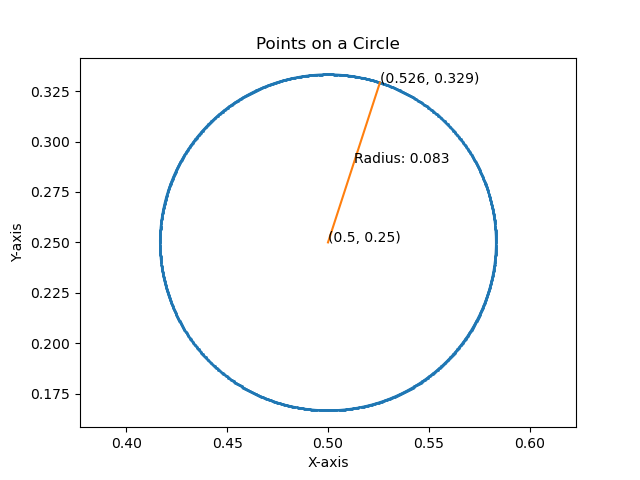
\includegraphics[width=0.7\linewidth]{figs/fig.png} % Ensure the image path is correct
   \caption{Equilateral triangle of side 5cm}
\end{figure}

\end{document}
